\documentclass{scrartcl}
\usepackage{amsmath}
\usepackage{graphicx}
\DeclareMathOperator*{\argminA}{arg\,min}

% Default fixed font does not support bold face
\DeclareFixedFont{\ttb}{T1}{txtt}{bx}{n}{12} % for bold
\DeclareFixedFont{\ttm}{T1}{txtt}{m}{n}{12}  % for normal

% Custom colors
\usepackage{color}
\definecolor{deepblue}{rgb}{0,0,0.5}
\definecolor{deepred}{rgb}{0.6,0,0}
\definecolor{deepgreen}{rgb}{0,0.5,0}

\usepackage{listings}

% Python style for highlighting
\newcommand\pythonstyle{\lstset{
language=Python,
breaklines=true,
basicstyle=\ttm,
otherkeywords={self},             % Add keywords here
keywordstyle=\ttb\color{deepblue},
emph={MyClass,__init__},          % Custom highlighting
emphstyle=\ttb\color{deepred},    % Custom highlighting style
stringstyle=\color{deepgreen},
frame=tb,                         % Any extra options here
showstringspaces=false            %
}}


% Python environment
\lstnewenvironment{python}[1][]
{
\pythonstyle
\lstset{#1}
}
{}

% Python for external files
\newcommand\pythonexternal[2][]{{
\pythonstyle
\lstinputlisting[#1]{#2}}}


\title{DRAW: A Recurrent Neural Network For Image Generation}
\subtitle{MEC 634 Final Project}
\author{Prerna Kothari}
\begin{document}
\maketitle
\abstract{
  This work is an implementation of a generative neural network architectures for image generation called \textbf{D}eep \textbf{R}ecurrent \textbf{A}ttentive \textbf{W}riter (DRAW).
DRAW network, developed by Google Deepmind team, combines a novel spatial attention mechanism that mimics the foveation of the human eye, with a sequential variational auto-encoding framework that allows for the iterative construction of complex images.
The system substantially improves on the state of the art for generative models on MNIST.
}

\section{Introduction}
This approach mimics human intuition of image creation.
For example, when a person asked to draw, paint or otherwise recreate a visual scene will naturally do so in a sequential, iterative fashion, reassessing their handiwork after each modification.
Rough outlines are gradually replaced by precise forms, lines are sharpened, darkened or erased, shapes are altered, and the final picture emerges.
Most approaches to automatic image generation, however, aim to generate entire scenes at once.
The network presented comes under the family of variational auto-encoder networks.

\subsection{Variational Auto-Encoder Problem Statement}
Given a dataset, capture the probability distribution of data and generate new data samples from the estimated probability distribution.
Also discover the salient features and efficiently internalize the essence of the data in order to generate it.

Let $\{x\}_i^N$ be the dataset consisting of N data points, where x is a d dimensional vector given by,
\begin{equation}
  x = \{ x_1, x_2, ... , x_d \}
\end{equation}

Let us assume that the observed data $\{x\}_i^N$ is generated by a model with $\theta$ parameters based on hidden variables $\{z\}_i^N$, where $z$ are l dimensional vectors and are distributed according to probability distribution P.
We only see x, but we would like to infer the characteristics of z. In other words, we’d like to compute $p(z|x)$.

\begin{equation}
  p(z|x) = \frac{p(x|z)p(z)}{p(x)}
\end{equation}

Unfortunately finding $(x)$ is quite difficult.

\begin{equation}
  p(x) = \int p(x|z) p(z) dz
\end{equation}

Usually, it turns out to be an intractable distribution.
We try to approximate $p(z|x)$ with a neural network, which we call an encoder neural network.
Output of the encoder neural network is $q(z|x)$ and we want it to be very close the actual $p(z|x)$.
Thus, we minimize the KL divergence between $p(z|x)$ and $q(z|x)$ given by,

\begin{equation}\label{kl}
  L_{z} =  KL(q(z|x)||p(z|x)) \\
\end{equation}

Also, we want accurate generation of the new data samples given $z$, which is generated by a neural network called Generator or Decoder.
The reconstruction loss in generation could be given either by least squared loss between input and generated input or the negative of log likelihood if the input is binary.

\begin{equation}\label{rec}
  L_{x} = (\hat{x} - x)^2 \text{ or } - \sum (x log(\hat{x}) + (1-x) log(1-\hat{x}))\\
\end{equation}

Objective is the find set of parameters $ \theta_{enc}, \theta_{dec}$ such that sum of mean reconstruction loss and KL divergence loss is minimum.
In other words,

\begin{equation}
  \argminA_{\theta_{enc}, \theta_{dec}} (L_{x}(\theta_{enc} + \theta_{dec}) + L_{z}(\theta_{enc})),
\end{equation}

Where, $\theta_{enc} $ are parameters of encoder network and $ \theta_{dec}$ are parameters of decoder network.

\section{DRAW Network}

The network presented in \cite{gregor2015draw} is a variational auto-encoder neural network with three main differences.
\begin{enumerate}
  \item {Firstly, both the encoder and decoder are recurrent networks in DRAW, so that a sequence
     of code samples is exchanged between them; moreover the encoder is privy to the decoder’s previous outputs, allowing
     it to tailor the codes it sends according to the decoder’s behavior so far.
     }

  \item {Secondly, the decoder’s outputs are successively added to the distribution that will ultimately generate
    the data, as opposed to emitting this distribution in a single step.
    }
  \item {Dynamically updated attention mechanism is used to restrict both the input region observed by the encoder,
    and the output region modified by the decoder.
    }

\end{enumerate}

\subsection{Network Architecture}

At each time-step $t$, the encoder receives input from both the image $x$ and from the previous decoder hidden vector $h^{dec}_{t−1}$.
The precise form of the encoder input depends on a read operation, which will be defined in the next section.  The output $h^{enc}_t$ of the encoder is used to parameterise a distribution $Q(Z_t|h^{enc}_t)$ over the latent vector $z_t$.
In our experiments the latent distribution is a diagonal Gaussian $N (Z_t|\mu_t, \sigma_t)$.

At each time-step a sample $z_t ∼ Q(Z_t|h^{enc}_t)$ drawn from the latent distribution is passed as input to the decoder.
The output $h^{dec}_t$ of the decoder is added (via a write operation, defined in the sequel) to a cumulative canvas matrix $ct$, which is ultimately used to reconstruct the image.

The total number of time-steps $T$ consumed by the network before performing the reconstruction is a free parameter that must be specified in advance.
For each image $x$ presented to the network, $c0$, $h^{enc}_0$ , $h^{dec}_0$ are initialised to learned biases, and the DRAW network iteratively computes the following equations for $t = 1 . . . , T:$
\begin{eqnarray}
  \hat{x}_t &=& x − Sigmoid(ct−1) \\
  r_t &=& read(x_t, \hat{x}_t, h^{dec}_{(t−1)} \label{read_op} \\
  h^{enc}_t &=& RNN_{enc}(h^{enc}_{t−1} , [rt, h^{dec}_{t−1}]) \\
  z_t &\sim& Q(Z_t|h^{enc}_t) \\
  h^{dec}_t &=& RNN_{dec}(h^{dec}_{t−1}, z_t) \\
  c_t &=& c_{t−1} + write(h^{dec}_t) \label{write_op}
\end{eqnarray}


\begin{figure}
\centering
  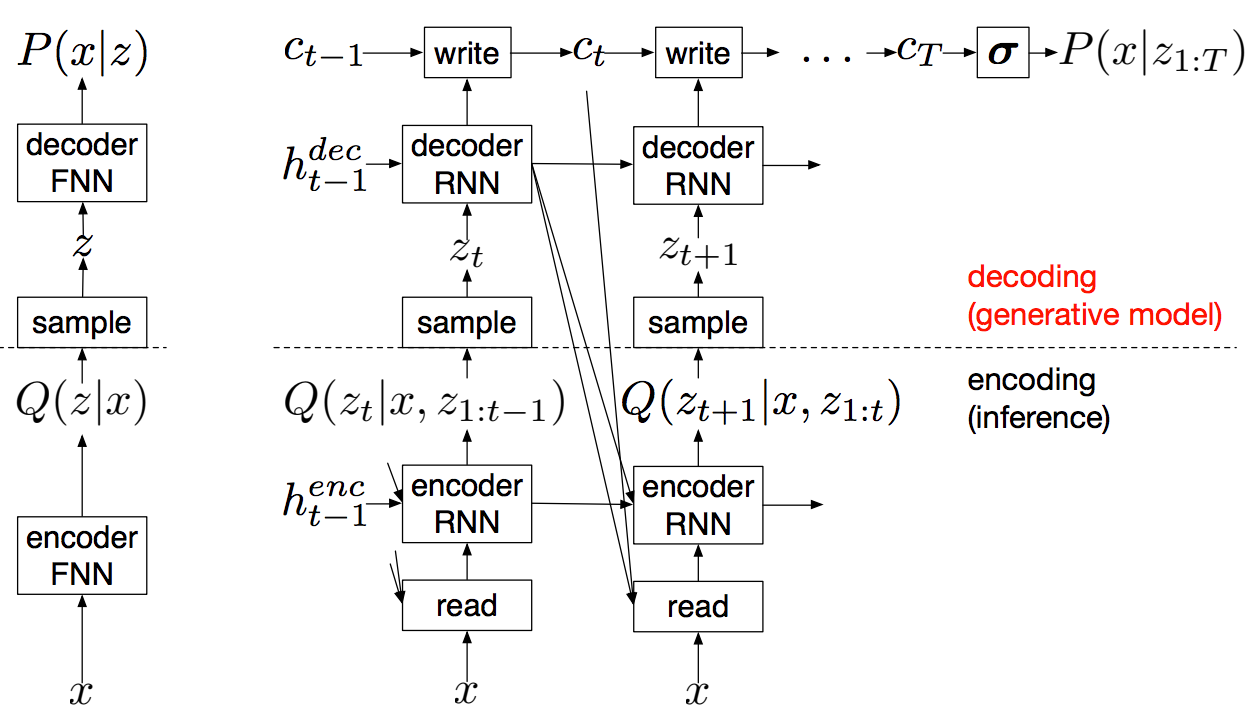
\includegraphics[width=350pt]{networkarch.png}
  \caption{\textbf{Left: Conventional Variational Auto-Encoder}. During generation, a sample z is drawn from a prior $P(z)$ and passed
through the feedforward decoder network to compute the probability of the input $P(x|z)$ given the sample. During inference the
input x is passed to the encoder network, producing an approximate posterior $Q(z|x)$ over latent variables. During training, z
is sampled from $Q(z|x)$ and then used to compute the total loss, which is minimised with stochastic gradient descent.
 \textbf{Right: DRAW Network}. At each time-step a sample $z_t$ from the prior $P(z_t)$ is passed to the recurrent decoder network, which then modifies part of the canvas matrix. The final canvas matrix $c_T$ is used to compute $P(x|z1:T)$. During inference the input is read at every timestep and the result is passed to the encoder RNN. The RNNs at the previous time-step specify where to read. The output of the encoder RNN is used to compute the approximate posterior over the latent variables at that time-step
  }
\label{network_arch}
\end{figure}

The loss functions for DRAW network as same as that of traditional variation auto-encoder.
The final image drawn at canvas is used for calculating reconstruction loss given in Eq.~\ref{rec}.
The KL divergence loss for Gaussian Distribution of $P(z)$ would be given by,

\begin{equation}\label{klg}
  L_{z} = \frac{1}{2} ( \sum^{T}_{t=1} {\mu^2}_t + {\sigma^2}_t - \log {\sigma^2}_t - T )
\end{equation}


\subsection{Stochastic Data Generation}
An image $\tilde{x}$ can be generated by a DRAW network by iteratively picking latent samples $\tilde{z}_t$ from the prior $P$, then running the decoder to update the canvas matrix $\tilde{c}_t$.
After T repetitions of this process the generated image is a sample from $D(X|\tilde{c}_T )$:

\begin{eqnarray}
  \tilde{z}_t &\sim& P(Zt) \\
  \tilde{h}^{dec}_t &=& RNN_{dec}(\tilde{h}^{dec}_{t−1}, \tilde{z}_t) \\
  \tilde{c}_t &=& \tilde{c}_{t−1} + write(\tilde{h}^{dec}_t) \\
  \tilde{x} &\sim& D(X|\tilde{c}_T)
\end{eqnarray}

\section{Read and Write Operations}
The DRAW network described in the previous section is
not complete until the read and write operations in Eqs.~\ref{read_op}
and~\ref{write_op} have been defined. This section describes two ways
to do so, one with selective attention and one without

\subsection{Reading and Writing without Attention}

In the simplest instantiation of DRAW the entire input image is passed to the encoder at every time-step, and the decoder modifies the entire canvas matrix at every time-step.
In this case the read and write operations reduce to,

\begin{eqnarray}
  read(x, \tilde{x}_t, h^{dec}_{t−1}) = [x, \tilde{x}_t] \\
  write(h^{dec}_t) = W(h^{dec}_t)
\end{eqnarray}

Where W is a linear weight matrix with weights and biases.

\subsection{Reading and Writing with Attention}
In order to allow model to have control over where to read, what to read and what to write, five parameters based on linear multiplication of decoder output are obtained. These five parameters are used to compute the patch origin $(g_x, g_y)$, path size $(\delta)$, isotropic Gaussian variance $\sigma_{var}$ and scalar intensity $\gamma$.

\begin{eqnarray}
  (\tilde{g_x}, \tilde{g_y} , \log\sigma^2 , \log\tilde{δ}, \log\gamma ) &=& W (h^{dec}) \\
  g_x &=& \frac{A + 1}{2} (\tilde{g_x} + 1) \\
  g_y &=& \frac{B + 1}{2} (\tilde{g_y} + 1) \\
  \delta &=& \frac{max(A, B) - 1}{N - 1} \tilde{\delta}
\end{eqnarray}

Using the Selective Attention machinery, we formulate read operation as follows,
\begin{equation}
  read(x, \tilde{x}_t, h^{dec}_{t−1}) = \gamma [F_Y x F^T_X , F^Y \hat{x} F^T_X ]
\end{equation}

Where, $F_X$ and $F_Y$ are filterbank matrices given by,
\begin{eqnarray}
  F_X[i, a] &=& \frac{1}{ZX} exp( - \frac{{(a - \mu^i_X)}^2}{ 2\sigma_{var}^2}) \\
  F_X[j, b] &=& \frac{1}{ZY} exp( - \frac{{(b - \mu^j_Y)}^2}{ 2\sigma_{var}^2})
\end{eqnarray}

Where, 1) $a$ and $b$ are indices from 1 to height and 1 to width respectively;
2) $i$ and $j$ are indices from 1 to $\tilde{\delta}$ respectively.
Also, the patch matrix $\mu$ is calculated is below:

For i is a row and j is a column of the patch,
\begin{eqnarray}
  \mu^i_X &=& g_x + (i - N/2 - 0.5)\delta \\
  \mu^j_Y &=& g_y + (j - N/2 - 0.5)\delta \\
\end{eqnarray}

\section{Results}
  The model is trained on MNIST dataset. Hyper parameters used are tabulated in Table \ref{hyper}.
  Figure~\ref{train} depicts the training losses with respect to number of training batches, where each batch consists of 100 images.

\begin{figure}
\centering
  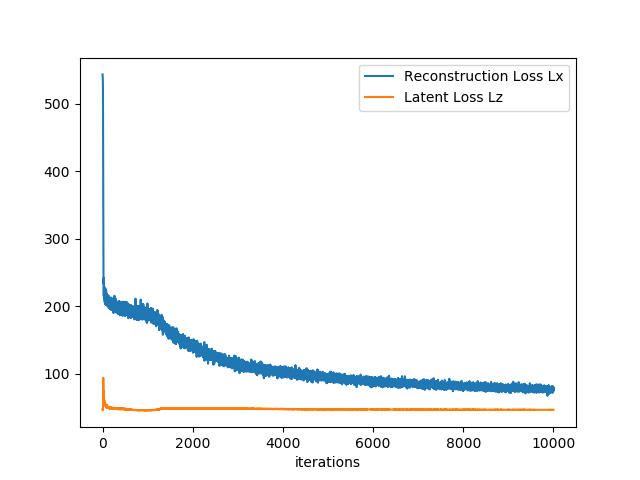
\includegraphics[width=300pt]{pre_loss.png}
  \caption{Training of DRAW Network. Two losses (Reconstruction and KL Divergence) compete with each other to find an equilibrium.}
\label{train}
\end{figure}

  The figures in Table~\ref{recon} depict the step-wise reconstruction of 16 MNIST images in 10 steps. It can be seen that the images are improved iterative fashion over ten steps. Thus it can be concluded that implementation is successful for iterative image generation with attention.

\begin{table}
\caption{DRAW Network Hyper Parameters}
\centering
\label{hyper}
\begin{tabular}{cc}
\hline
Learning Rate & 0.001 \\
Batch Size & 100 \\
Total Time Steps $(T)$ & 10 \\
Encoder Hidden Units & 128 \\
Decoder Hidden Units & 128 \\
Latent Dimension & 10 \\
\hline
\end{tabular}
\end{table}

\begin{table}
\caption{Step Wise Reconstruction}
\centering
\label{recon}
\begin{tabular}{cc}
\hline
$t_0$ 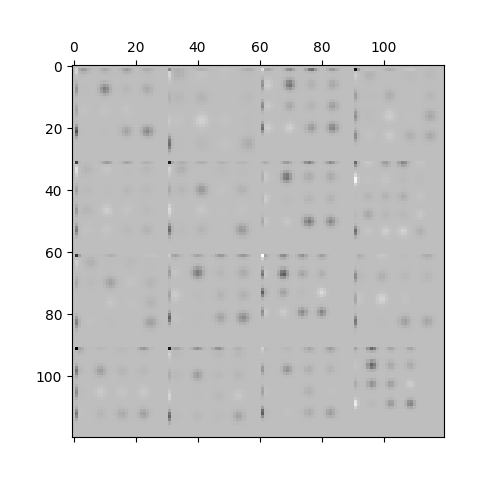
\includegraphics[width=140pt]{new_0.png} & $t_1$ 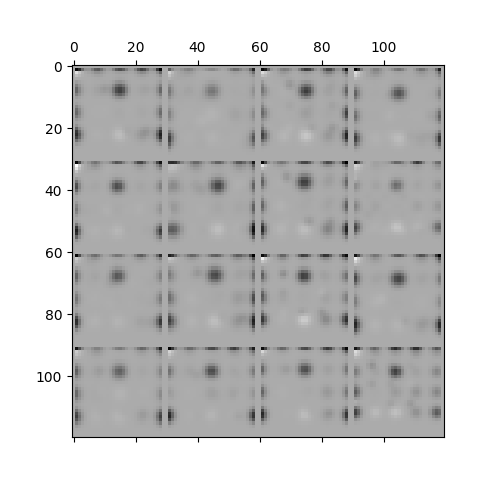
\includegraphics[width=140pt]{new_1.png}\\
$t_2$ 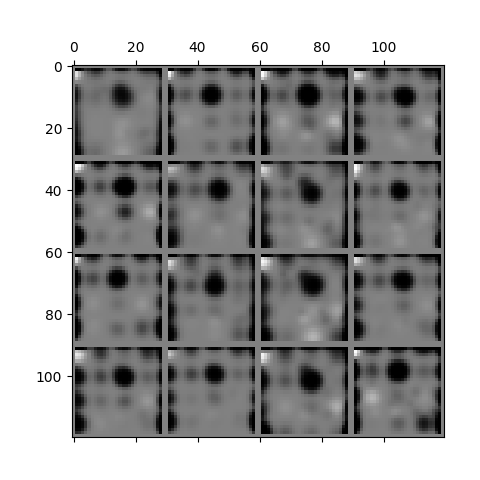
\includegraphics[width=140pt]{new_2.png} & $t_3$ 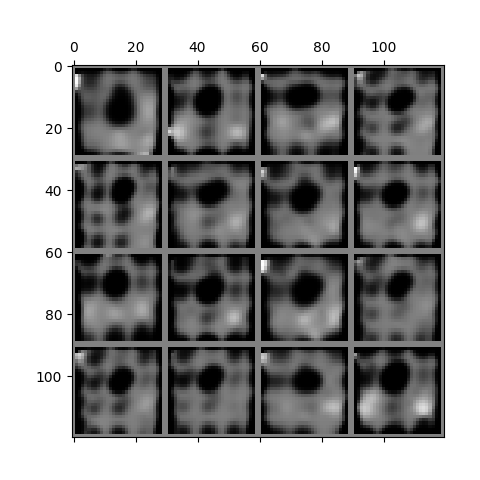
\includegraphics[width=140pt]{new_3.png}\\
$t_4$ 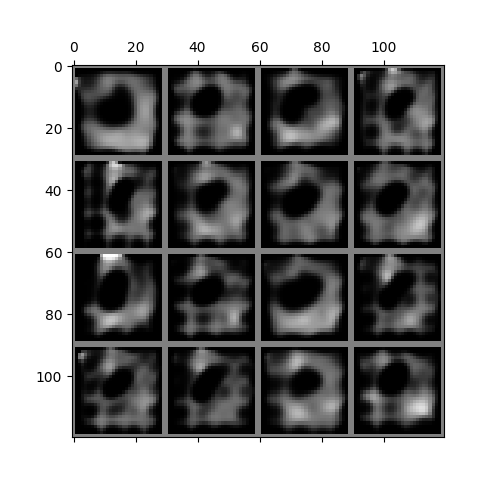
\includegraphics[width=140pt]{new_4.png} & $t_5$ 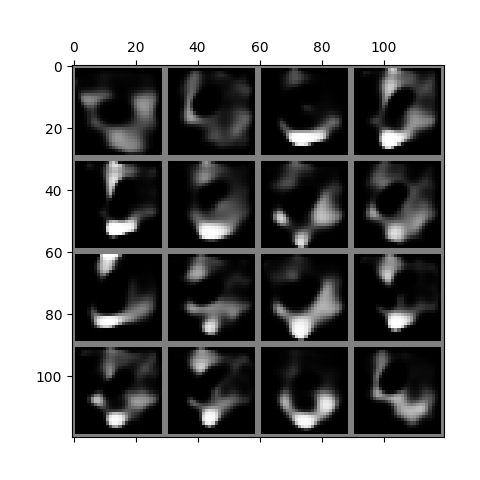
\includegraphics[width=140pt]{new_5.png}\\
$t_6$ 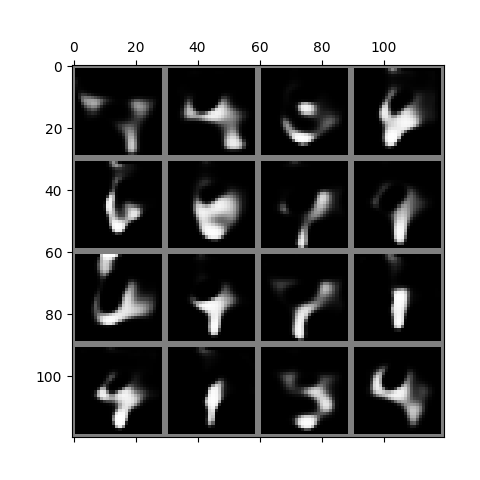
\includegraphics[width=140pt]{new_6.png} & $t_7$ 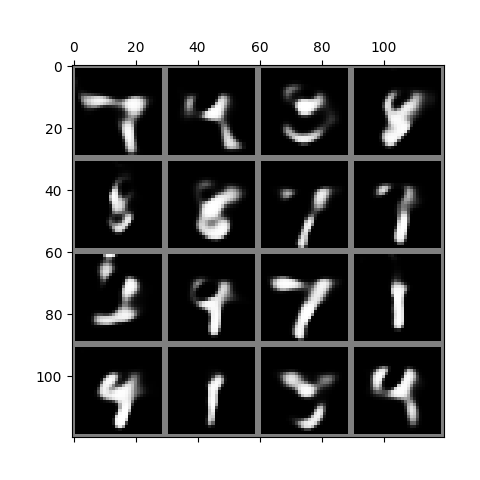
\includegraphics[width=140pt]{new_7.png}\\
$t_8$ 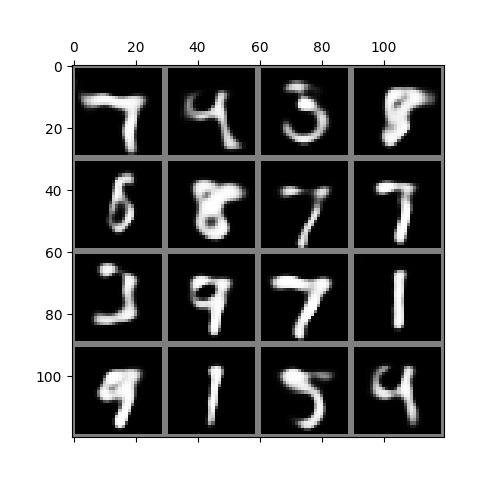
\includegraphics[width=140pt]{new_8.png} & $t_9$ 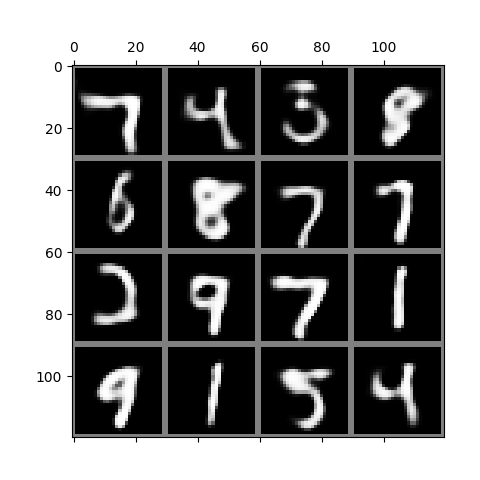
\includegraphics[width=140pt]{new_9.png}\\
\hline
\end{tabular}
\end{table}


\bibliographystyle{purwar}
\bibliography{references}

\section{Appendix: Python Code}

\pythonexternal{model.py}

\end{document}
